\begin{comment}
Vorbereiten der Suche
\begin{itemize}
    \item Es sollen mögliche Medienformate untersucht werden.
\end{itemize}

\paragraph{Result} \hfill \\
Analyse der möglichen Medienformate und Entscheid für ein bis zwei Formate für die Indizierung.
\end{comment}


\chapter{Metadaten Aufbereiten}
\label{ch:formats}

In der Media Library sind MP3 und FLAC Dateien weitaus
am häufigsten vorhanden, weshalb wir nur diese beiden Audioformate
genauer betrachten werden. Aus den Metadaten dieser
Audioformate interessiert uns vor allem das Tag, die
Metadaten zum Audio Track, wie der Interpret, der Titel
oder das Album.

Um die Metadaten der Mediadateien zu betrachten und
zu editieren, verwenden wir der Einfachheit halber das Tool
EasyTAG \cite{web:easytag}. Dieses Tool ist verfügbar für
Linux und weitere Platformen, es ist intuitiv zu bedienen.
Neben den Attributen sehen wir darin zum Beispiel in
\cref{fig:easytag} auch, dass die Metadaten der gewählten
Datei als  Vorbis Tag gespeichert sind.

\begin{figure}[ht]
    \centering
    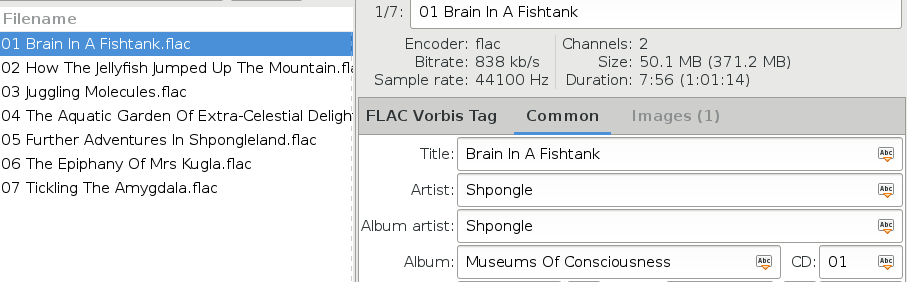
\includegraphics[width=\textwidth]{easytag}
    \caption{Metadaten mit EasyTAG editieren}
    \label{fig:easytag}
\end{figure}

\section{MP3 Format}
MPEG-1 oder MPEG-2 Audio Layer {III} allgemein bekannt als MP3
ist ein verlustbehafteteter Audio Codec. Die
\href{http://mpeg.chiariglione.org/}{Movie Pictures Expert Group}
(MPEG) hat dieses Format entworfen.
MP3 Dateien können aus mehreren Frames bestehen, ein
solches Frame enthält jeweils einen MP3 Header und MP3 Daten.
Der Header enthält Informationen wie zum Beispiel das Format,
die Version des Formates oder die Bitrate. Der MP3 Standard
enthält offiziell keinen Container für Tags. Üblicherweise werden
Tags im ID3v1 oder ID3v2 Format an MP3 Dateien gehängt.
ID3v1 ist ein \(128\) Byte langer Block welcher wie in 
\cref{tab:id3v1}
aufgebaut ist. Dieser Block enthält minimale Metadaten
über das in der MP3 Datei gespeicherte Stück.

\begin{table}[ht]
    \centering
    \begin{tabu}{l|l|l}
        \hline
        \rowfont[c]{\bfseries} Feld & Bytes & Beschreibung \\
        \hline
        header    & 3           & "TAG" \\
        title     & 30          & \\
        artist    & 30          & \\
        album     & 30          & \\
        year      & 4           & \\
        comment   & 28 oder 30  & Optional, letzte 2 Bytes für Track Nr. \\
        zero-byte & 1           & Enthält 0, falls Track Nr. vorhanden \\
        track     & 1           & Track Nr. falls zero-byte gesetzt \\
        genre     & 1           & Index in einer Liste möglicher Genres, sonst 255
    \end{tabu}
    \caption{ID3v1 Layout}
    \label{tab:id3v1}
\end{table}

Im Gegensatz zu ID3v1 hat der ID3v2 keine fixe, sondern eine
variable Länge. In einem ID3v2 können sehr viel mehr Attribute
gespeichert werden, es existiert selbst für Bildcover ein
Attribut. \cite{wiki:mp3,wiki:id3}

\section{FLAC Format}
Free and Lossless Audio Codec (FLAC) ist ein verlustfreier
Audio Codec. FLAC ist ein offenes Format und steht unter
der \href{http://www.gnu.org/licenses/gpl.html}{GNU General Public License}.
Die grundlegende Struktur einer FLAC Datei ist wie folgt aufgebaut.
\cite{web:flac}

\begin{itemize}[noitemsep]
    \item \emph{flac} als String
    \item Block mit Metadaten zu Samplerate, Anzahl Channels etc.
    \item Keinen oder mehrere Metadaten Blocks, ein Block kann ein Bild, Vorbis Kommentar oder Track Informationen enthalten.
    \item Eines oder mehrere Audioframes.
\end{itemize}

Der Standard sieht den Vorbis Comment für die Tag Metadaten vor.
Dieser Standard lässt zu, bis zu \(2^{24}\) Bytes in einem
Vorbis Comment zu speichern. Die Daten sollen in
menschenlesbarem Format gespeichert werden, damit entfallen
Probleme wie zum Beispiel das Genre im ID3 Tag Format,
welches nur als Index gespeichert wird. Um aus diesem
Index das Genre zu erhalten, muss man die überall gleiche
Liste aller Genres kennen. \cite{web:vorbiscomment}

\section{Metadaten Parsen}
\label{sec:parse}
Um die Metadaten zu den unterschiedlichen Audioformaten
zu parsen wird die Library Apache Tika \cite{web:tika}
verwendet. Diese Library bietet für verschiedenste
Dokumente, darunter Textdokument, Source Code Dateien
oder eben auch Media Dateien, Parser um aus den Dateien
Metainformationen zu extrahieren.\cite{web:tikaformats}

Mit dem \href{https://tika.apache.org/1.13/api/org/apache/tika/parser/mp3/Mp3Parser}{MP3Parser}
können Metadaten aus MP3 Dateien
extrahiert werden. Für FLAC Dateien existiert der
externe \href{https://github.com/Gagravarr/VorbisJava/blob/master/tika/src/main/java/org/gagravarr/tika/FlacParser.java}{FlacParser}
aus dem \href{https://github.com/Gagravarr/}{Gagravarr Package}.
Tika bietet mit dem
\href{https://tika.apache.org/1.13/api/org/apache/tika/parser/AutoDetectParser.html}{AutoDetectParser}
zusätzlich einen Parser, welcher einem den Umstand abnimmt
selbst entscheiden zu müssen, welcher Parser für eine
bestimmte Datei verwendet werden soll. Wir werden
nachfolgend nur mit diesem Parser arbeiten.

In nachfolgenden Listing sehen wir wie wir den Parser
verwenden um damit die \emph{metadata} aus dem
\emph{file} zu extrahieren.

\begin{lstlisting}[style=myScalastyle]
val metadata = new Metadata
val handler  = new BodyContentHandler
val context  = new ParseContext
val parser   = new AutoDetectParser
val stream   = Try(new FileInputStream(file))

stream.map( s =>
    catching(classOf[TikaException],
             classOf[SAXException])
    andFinally(s.close())
    withTry(parser.parse(s, handler, metadata, context))
) match {
    case Success(_) =>
        return metadata
    case Failure(e:Throwable) => println(e.toString())
}
\end{lstlisting}

\begin{table}[ht]
    \centering
    \begin{tabu}{l|l}
        \hline
        \rowfont[c]{\bfseries} Attribut & Wert \\
        \hline
        xmpdm:genre            & Hardstyle \\
        x-parsed-by            & org.apache.tika.parser.DefaultParser \\
        creator                & Showtek \\
        xmpdm:album            & Today is Tomorrow \\
        xmpdm:tracknumber      & 05 \\
        xmpdm:releasedate      & 2007 \\
        meta:author            & Showtek \\
        xmpdm:artist           & Showtek \\
        dc:creator             & Showtek \\
        xmpdm:audiocompressor  & MP3 \\
        title                  & FTS \\
        xmpdm:audiochanneltype & Stereo \\
        version                & MPEG 3 Layer III Version 1 \\
        xmpdm:audiosamplerate  & 44100 \\
        channels               & 2 \\
        dc:title               & FTS \\
        author                 & Showtek \\
        xmpdm:duration         & 165467.921875 \\
        content-type           & audio/mpeg \\
        samplerate             & 44100
    \end{tabu}
    \caption{Metadaten einer MP3 Datei}
    \label{tab:tikameta}
\end{table}

Die Metadaten zu einer von unseren Audiodateien
sehen wir in \cref{tab:tikameta}.
Unter diesen Attributen fällt auf, dass viele mit
\emph{xmpdm} beginnen. Bezeichner vor dem Doppelpunkt
sind Formate in welchen Tika dieses Attribut ablegt.
\emph{xmpdm} steht für XMP Digital Media.
Extensible Metadata Platform (XMP)
ist ein Standard für den Austausch von Metadaten.\cite{wiki:xmp}

Im nachfolgende Kapitel werden wir die Attribute \emph{xmpdem:genre},
\emph{author}, \emph{xmpdm:releasedate}, \emph{title}
und \emph{xmpdmalbum} indizieren.